\documentclass{article}%文档类型
\usepackage[UTF8]{ctex}%允许中文
\usepackage[a4paper,left=10mm,right=10mm,top=15mm,bottom=15mm]{geometry}%文档布局
\usepackage{titling}%标题包
\usepackage{xcolor}%颜色包
\usepackage{listings}%代码显示包
\usepackage{float}
\usepackage{array}
\usepackage{graphicx}%图像插入包
\usepackage{multirow}
\graphicspath{{../image/}}
\renewcommand{\arraystretch}{2} % 增加整体行高
\usepackage{appendix}
\usepackage{hyperref}



%代码显示设置
\lstset{
    language=Python, % 设置语言
    basicstyle={\small\ttfamily}, % 设置字体族
    breaklines=true, % 自动换行
    keywordstyle=\color{blue},  % 关键字样式
    commentstyle=\color{green}, % 注释样式
    stringstyle=\color{red},    % 字符串样式
    emph={self},           % 添加强调词
    emphstyle=\color{blue}\bfseries, % 强调词样式
    columns=flexible,
    numbers=left, % 显示行号在左边
    numbersep=2em, % 设置行号的具体位置
    numberstyle=\footnotesize, % 缩小行号
    frame=single, % 边框
    framesep=1em, % 设置代码与边框的距离
    xleftmargin=2em, % 左边距
    xrightmargin=2em, % 右边距
}

\title{视听信息系统导论第一次编程作业报告}

\begin{document}
%标题页
\begin{titlepage}
    \thispagestyle{empty}
    \vspace*{4cm} % 顶部填充
    \begin{center}
    {\LARGE \textbf{\thetitle}}\\
    \vspace{6cm}
    \end{center}
    \vspace*{\fill} % 底部填充
\end{titlepage}

\zihao{-4}
\setlength{\baselineskip}{22pt}
\tableofcontents
\clearpage



\section{实验内容}
\subsection{构建结构如下的神经网络,在层与层之间使用 tanh 激活函数,
不使用 BatchNorm,使用SGD 优化器,完成 CIFAR10 图像分类任务,绘制出训练、
测试时的损失曲线,并绘制准确率变化图像。}

实验中使用tanh激活函数,不使用BatchNorm,完成测试任务后得到的曲线如下:
\begin{figure}[H]
    \centering
    \begin{minipage}{0.49\linewidth}
        \centering
        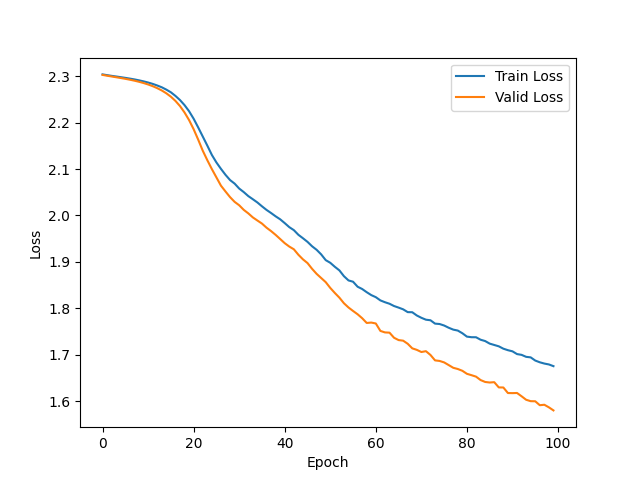
\includegraphics[width=0.9\linewidth]{Loss_1.png}
        \caption{Loss曲线}
    \end{minipage}
    \begin{minipage}{0.49\linewidth}
        \centering
        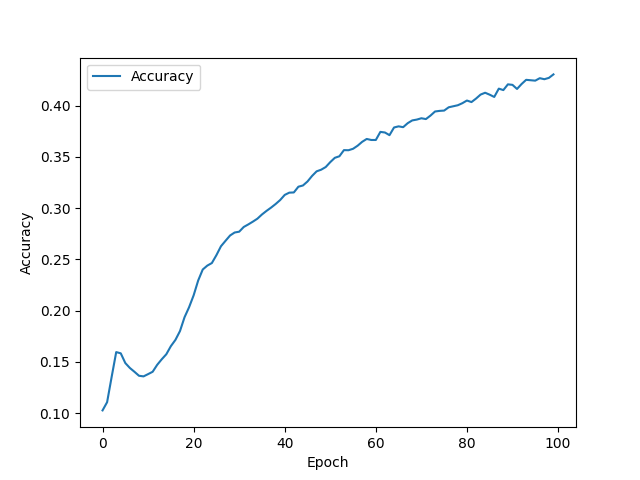
\includegraphics[width=0.9\linewidth]{Acc_1.png}
        \caption{Accuracy曲线}
    \end{minipage}
\end{figure}

\subsection{仍然使用上述网络结构,将激活函数更改为 ReLU 函数,并使用 BatchNorm,使用 SGD
优化器,完成 CIFAR10 图像分类任务,绘制出训练、测试时的损失曲线,并绘制准确率
变化图像。}

实验中激活函数使用ReLU,并且使用BatchNorm,完成测试任务后得到的曲线如下:
\begin{figure}[H]
    \centering
    \begin{minipage}{0.49\linewidth}
        \centering
        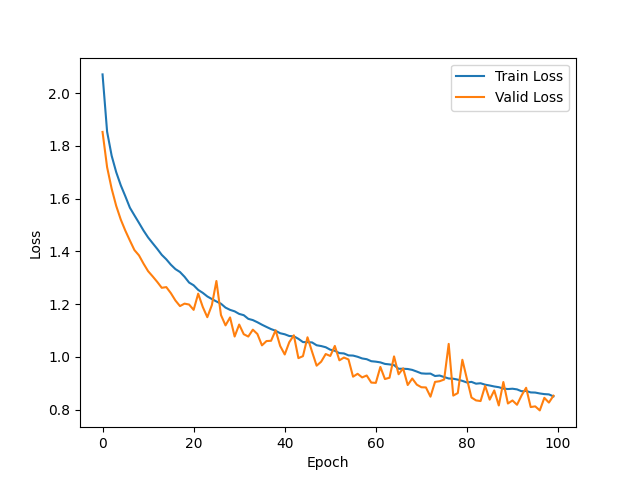
\includegraphics[width=0.9\linewidth]{Loss_2.png}
        \caption{Loss曲线}
    \end{minipage}
    \begin{minipage}{0.49\linewidth}
        \centering
        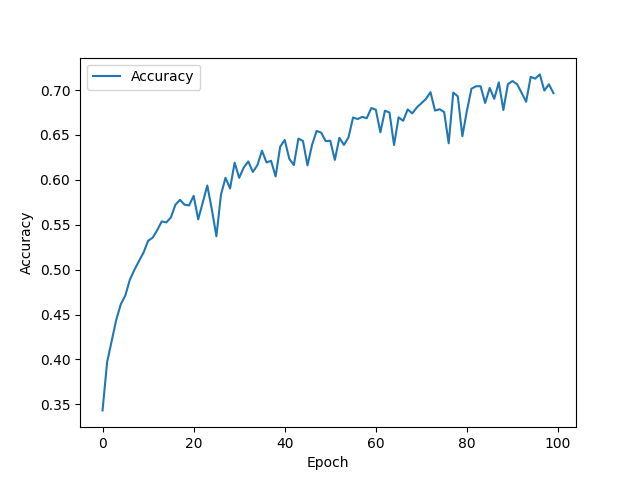
\includegraphics[width=0.9\linewidth]{Acc_2.png}
        \caption{Accuracy曲线}
    \end{minipage}
\end{figure}

\subsection{在 2 的基础上,将优化器换为 Adam 优化器,完成 CIFAR10 图像分类任务,绘制出训
练、测试时的损失曲线,并绘制准确率变化图像。}
在2的基础上,使用Adam优化器,完成测试任务后得到的曲线如下:
\begin{figure}[H]
    \centering
    \begin{minipage}{0.49\linewidth}
        \centering
        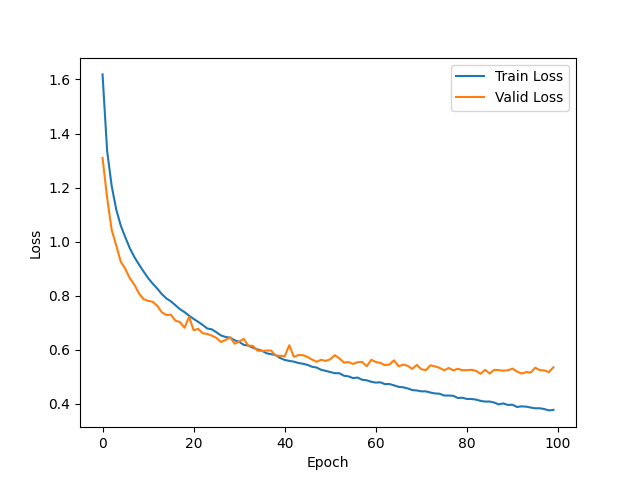
\includegraphics[width=0.9\linewidth]{Loss_3.png}
        \caption{Loss曲线}
    \end{minipage}
    \begin{minipage}{0.49\linewidth}
        \centering
        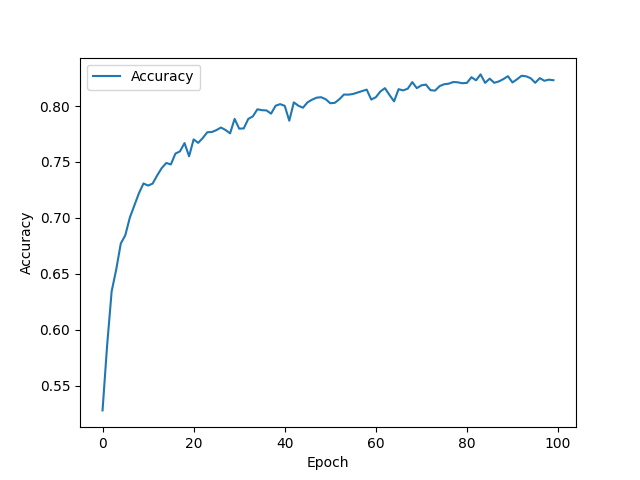
\includegraphics[width=0.9\linewidth]{Acc_3.png}
        \caption{Accuracy曲线}
    \end{minipage}
\end{figure}

\subsection{构建规定的神经网络,重复 1 到 3 的任务。}
构建指导书中的神经网络,重复任务1到3得到的图像如下:

\begin{figure}[H]
    \centering
    \begin{minipage}{0.49\linewidth}
        \centering
        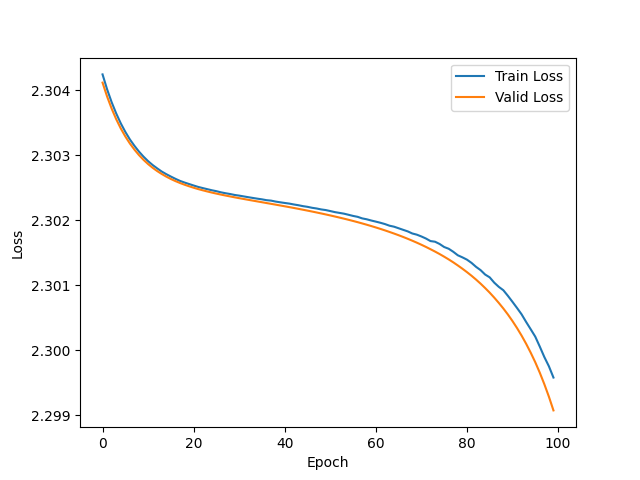
\includegraphics[width=0.9\linewidth]{Loss_4.png}
        \caption{任务1 Loss曲线}
    \end{minipage}
    \begin{minipage}{0.49\linewidth}
        \centering
        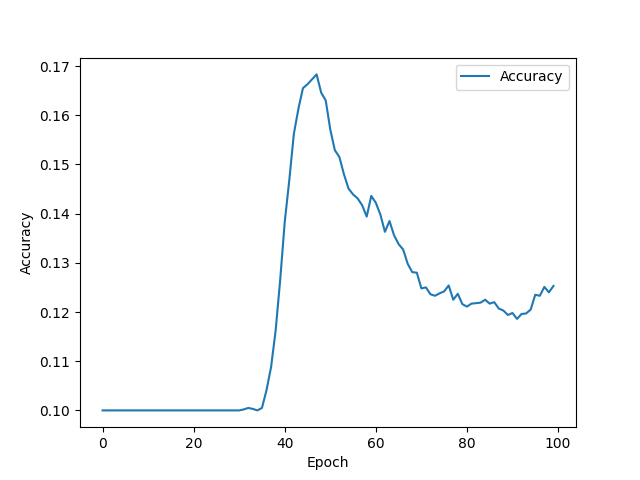
\includegraphics[width=0.9\linewidth]{Acc_4.png}
        \caption{任务1 Accuracy曲线}
    \end{minipage}
\end{figure}

\begin{figure}[H]
    \centering
    \begin{minipage}{0.49\linewidth}
        \centering
        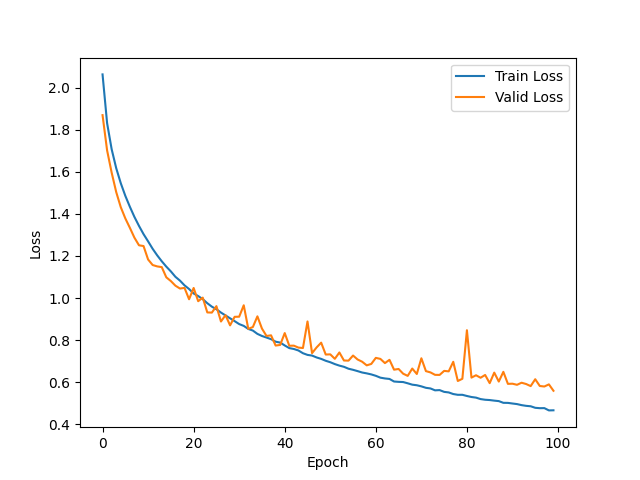
\includegraphics[width=0.9\linewidth]{Loss_5.png}
        \caption{任务2 Loss曲线}
    \end{minipage}
    \begin{minipage}{0.49\linewidth}
        \centering
        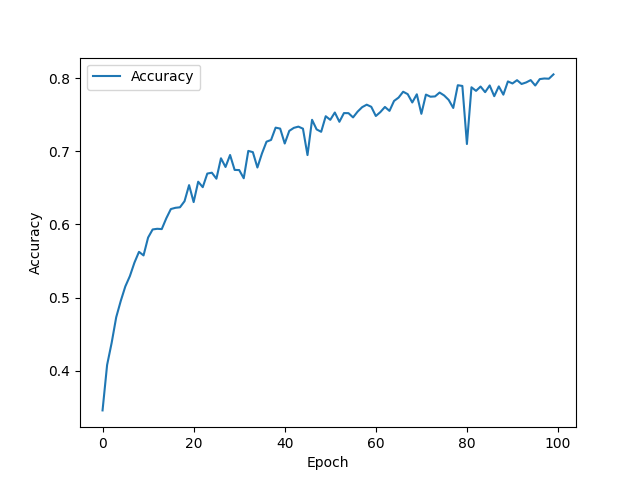
\includegraphics[width=0.9\linewidth]{Acc_5.png}
        \caption{任务2 Accuracy曲线}
    \end{minipage}
\end{figure}

\begin{figure}
    \centering
    \begin{minipage}{0.49\linewidth}
        \centering
        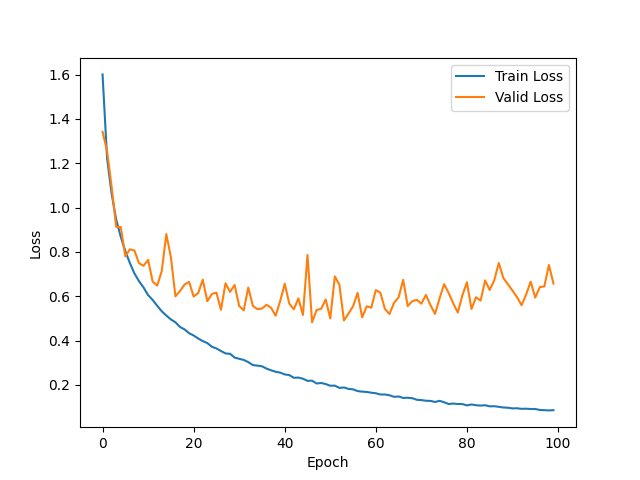
\includegraphics[width=0.9\linewidth]{Loss_6.png}
        \caption{任务3 Loss曲线}
    \end{minipage}
    \begin{minipage}{0.49\linewidth}
        \centering
        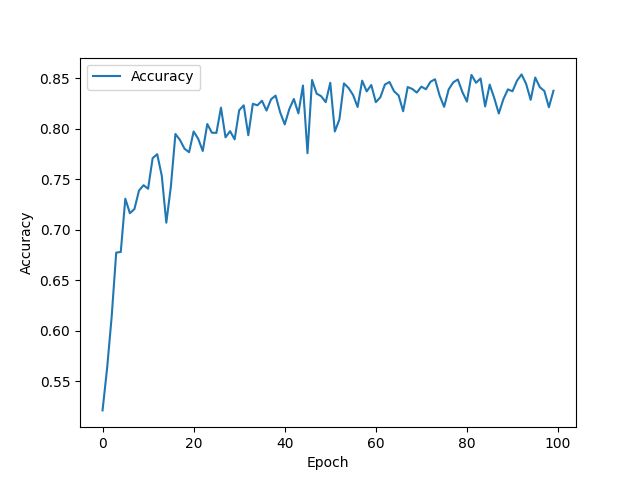
\includegraphics[width=0.9\linewidth]{Acc_6.png}
        \caption{任务3 Accuracy曲线}
    \end{minipage}


\end{figure}

\section{结果分析}
\subsection{请根据结果分析 ReLU 和 tanh 激活函数的表现}
由于题目要求没有控制变量(2中将激活函数更改为ReLU函数的同时使用了BatchNorm),变量改变不唯一。
因此我们另外测试了只将激活函数更改为 ReLU 函数的情况,以及在使用BatchNorm时将tanh作为激活函数函数的情况,
此时变量是唯一的,更有助于我们研究不同激活函数造成的影响。通过实验得到的测试结果如下表:

\begin{table}[H]
    \centering
    \begin{tabular}{|m{2cm}|m{1cm}|m{0.3\linewidth}|m{0.3\linewidth}|}
        \hline
        BatchNorm \newline 函数 &模型 &使用tanh函数激活 &使用ReLU函数激活\\[0.5cm]
        \hline
        \multirow{2}{*}[-11ex]{\hspace{10pt}不使用}
        &\begin{center} 1 \end{center}  &\vspace{5pt} 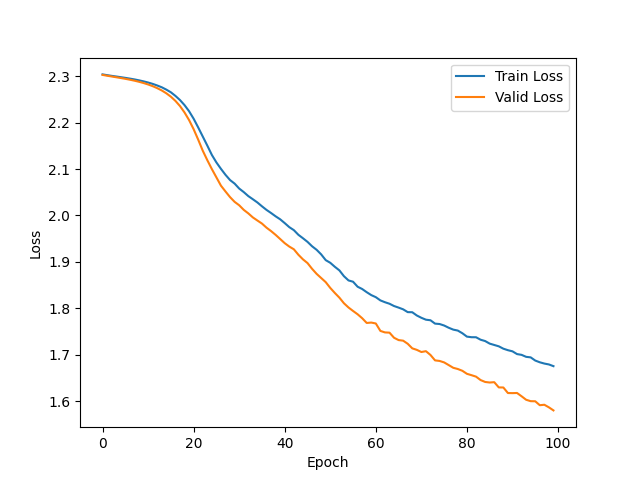
\includegraphics[width=1\linewidth]{Loss_1.png} &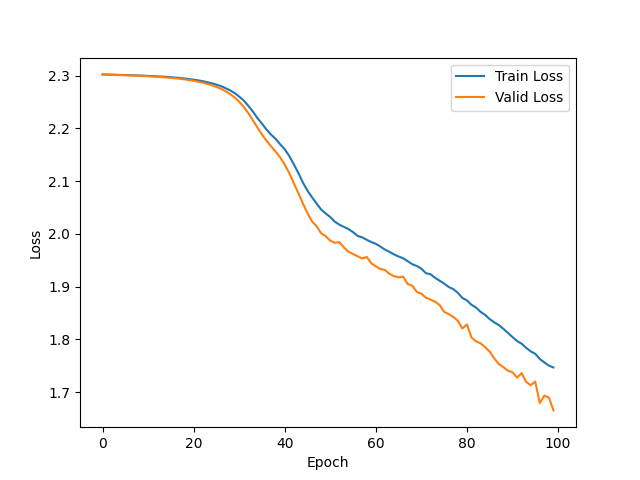
\includegraphics[width=1\linewidth]{Loss_1.5.png}  \\[0.6cm]
        \cline{2-4}
        &\begin{center} 2 \end{center}  &\vspace{5pt} 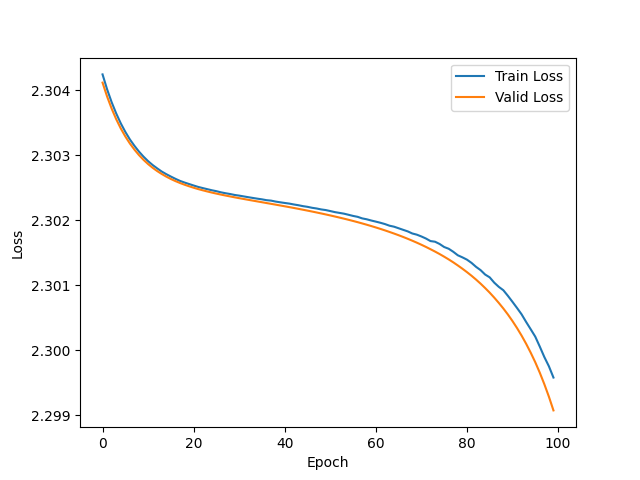
\includegraphics[width=1\linewidth]{Loss_4.png} &\vspace{5pt} 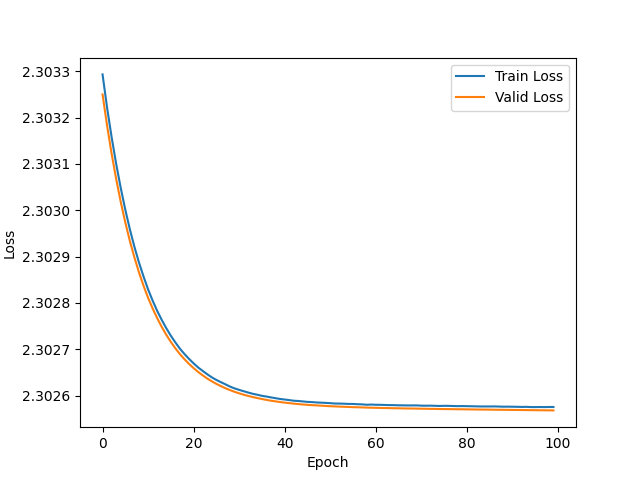
\includegraphics[width=1\linewidth]{Loss_4.5.png} \\[0.6cm]
        \hline
        \multirow{2}{*}[-11ex]{\hspace{14pt}使用}
        &\begin{center} 1 \end{center}  &\vspace{5pt} 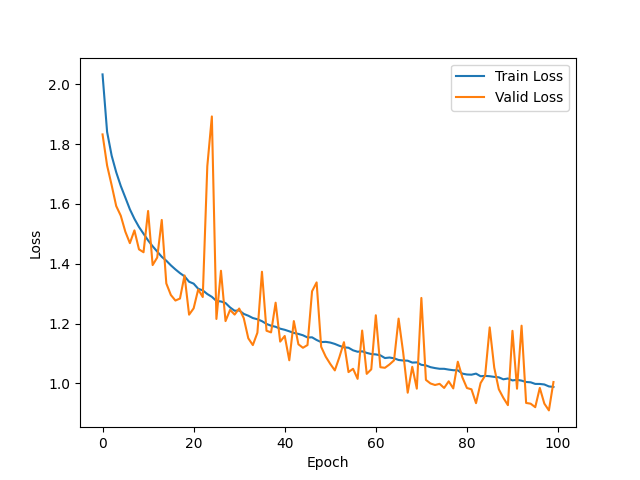
\includegraphics[width=1\linewidth]{Loss_2.5.png} &\vspace{5pt} 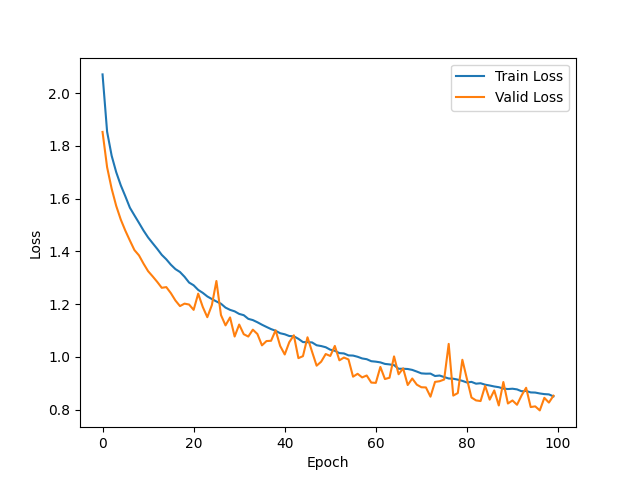
\includegraphics[width=1\linewidth]{Loss_2.png}  \\[0.6cm]
        \cline{2-4}
        &\begin{center} 2 \end{center}  &\vspace{5pt} 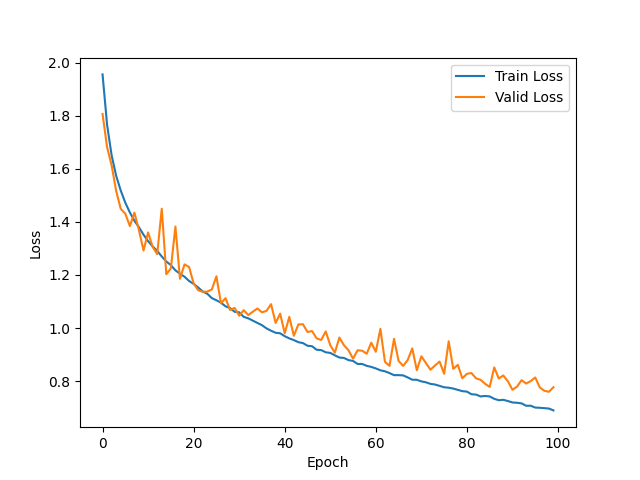
\includegraphics[width=1\linewidth]{Loss_5.5.png} &\vspace{5pt} 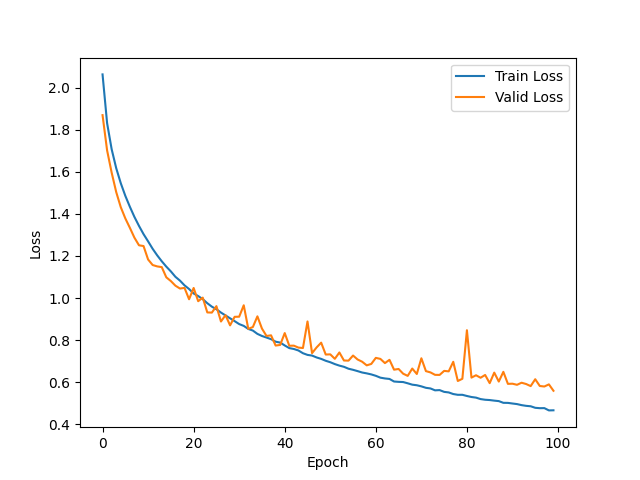
\includegraphics[width=1\linewidth]{Loss_5.png} \\[0.6cm]
        \hline
    \end{tabular}
    \caption{ReLU和tanh激活函数的不同表现——Loss曲线}
\end{table}

\begin{table}[H]
    \centering
    \begin{tabular}{|m{2cm}|m{1cm}|m{0.3\linewidth}|m{0.3\linewidth}|}
        \hline
        BatchNorm \newline 函数 &模型 &使用tanh函数激活 &使用ReLU函数激活\\[0.5cm]
        \hline
        \multirow{2}{*}[-11ex]{\hspace{10pt}不使用}
        &\begin{center} 1 \end{center}  &\vspace{5pt} 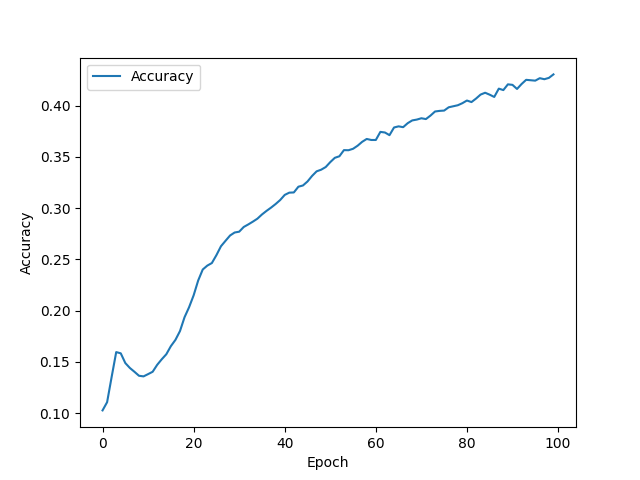
\includegraphics[width=1\linewidth]{Acc_1.png} &\vspace{5pt} 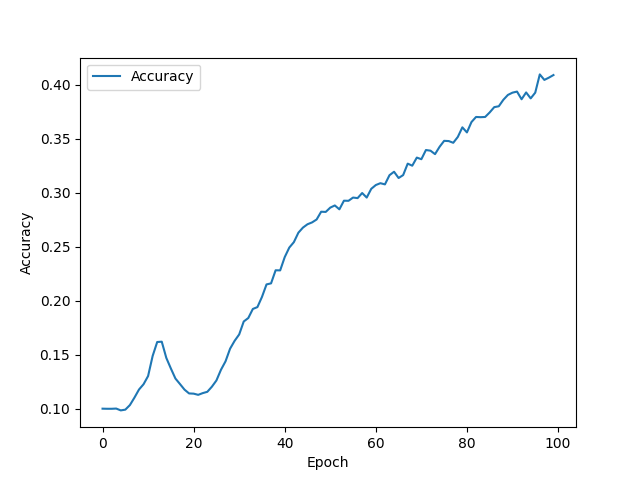
\includegraphics[width=1\linewidth]{Acc_1.5.png}  \\[0.6cm]
        \cline{2-4}
        &\begin{center} 2 \end{center}  &\vspace{5pt} 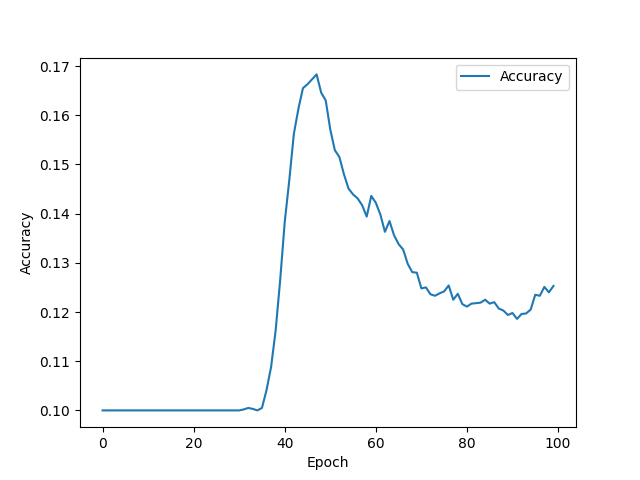
\includegraphics[width=1\linewidth]{Acc_4.png} &\vspace{5pt} 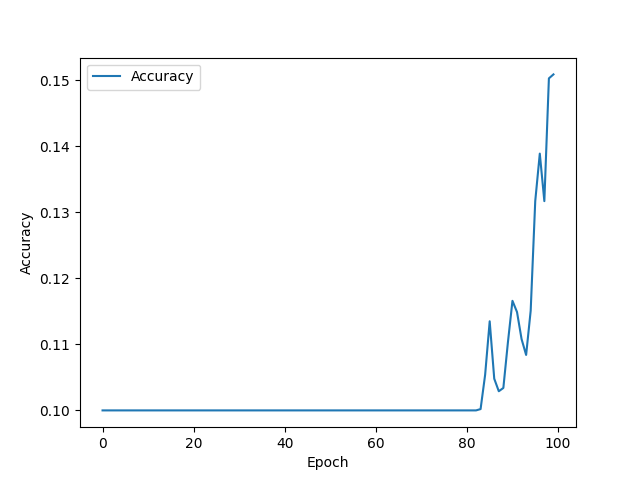
\includegraphics[width=1\linewidth]{Acc_4.5.png} \\[0.6cm]
        \hline
        \multirow{2}{*}[-11ex]{\hspace{14pt}使用}
        &\begin{center} 1 \end{center}  &\vspace{5pt} 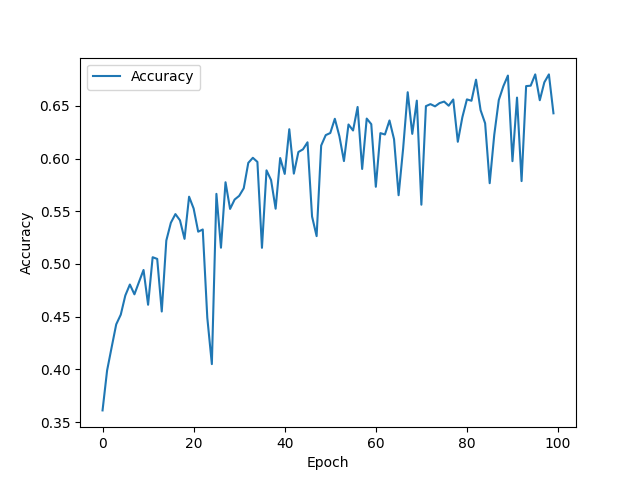
\includegraphics[width=1\linewidth]{Acc_2.5.png} &\vspace{5pt} 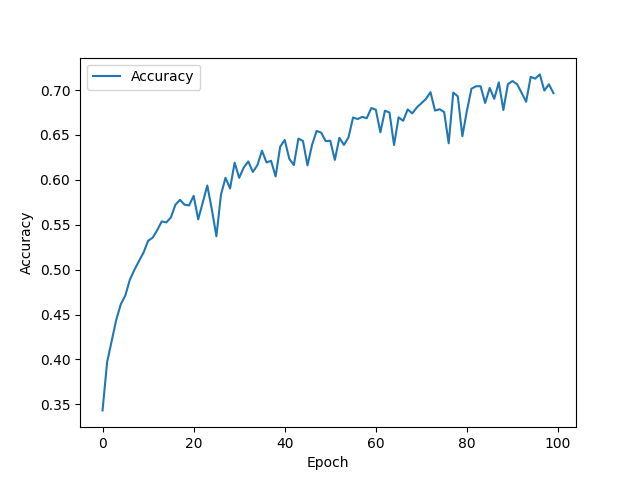
\includegraphics[width=1\linewidth]{Acc_2.png}  \\[0.6cm]
        \cline{2-4}
        &\begin{center} 2 \end{center}  &\vspace{5pt} 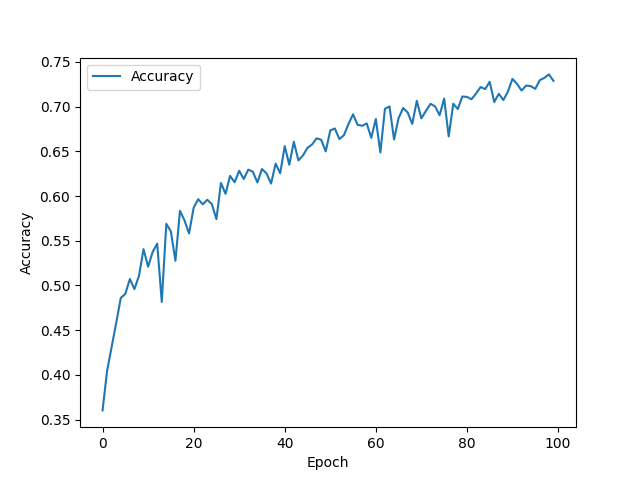
\includegraphics[width=1\linewidth]{Acc_5.5.png} &\vspace{5pt} 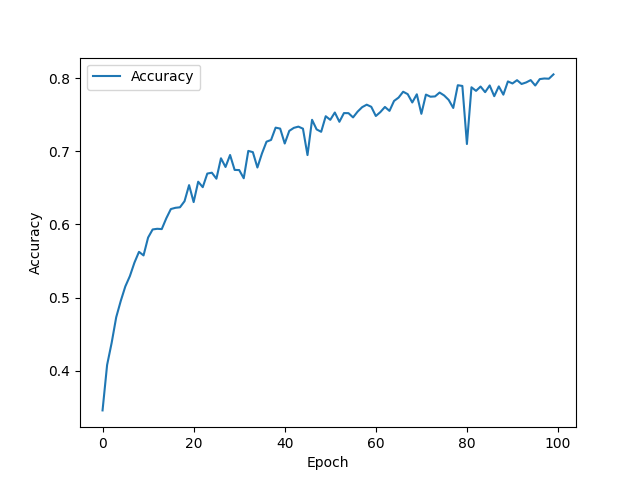
\includegraphics[width=1\linewidth]{Acc_5.png} \\[0.6cm]
        \hline
    \end{tabular}
    \caption{ReLU和tanh激活函数的不同表现——Accuracy曲线}
\end{table}

横向对比可以看到在其他条件均相同的情况下,不同激活函数对实验产生的影响。如果从简单的单变量的角度进行分析的话,
在不使用 BatchNorm 的情况下,单独换用 ReLU 和 tanh 激活函数,模型1差异不大,模型2中ReLU函数会让Loss的减小更加迅速
。而在加上 BatchNorm 后,ReLU 激活函数的模型在训练集和测试集上的表现略微更好一些,但是数值上的差异不大。

但是如果考虑到激活函数的特点不同(BatchNorm可以做归一化为零均值和单位方差,tanh激活函数输出的值本身就是归一化的)。
当ReLU激活函数同时使用BatchNorm时,可以看到ReLU激活函数在各方面的表现都要优于tanh函数,ReLU函数相较于tanh函数来说
,Loss曲线下降速度更快,更快到达稳定,稳定时Loss的值会更小。而且使用ReLU做激活函数,正确率也会更高,趋于稳定的速度更快,
同时可以明显看到在模型深度比较深的情况下,tanh函数激活准确率会出现明显的下降现象,而使用ReLU做激活函数则没有这种现象。

主要的原因可能是因为:
\begin{enumerate}
    \item ReLU的优点在于其计算简单、在正区间保持线性,有助于解决梯度消失问题,
    并且在稀疏激活时表现良好。缺点是在负区间值恒定为0,可能出现“死神经元”,永远输出0。
    \item tanh的优点在于输出范围更为平衡(-1到1),有助于中心化数据,
    但在深层网络中可能导致梯度消失,影响学习速度。
\end{enumerate}

\subsection{请根据结果分析 BatchNorm 的作用}
和讨论1中相似,我们同样使用控制变量法将变量控制为单一的是否使用BatchNorm,从而得到的训练结果如下:

\begin{table}[H]
    \centering
    \begin{tabular}{|m{1cm}|m{0.3\linewidth}|m{0.3\linewidth}|}
        \hline
        模型 &不使用BatchNorm函数 &使用BatchNorm函数\\[0.5cm]
        \hline
        \begin{center} 1 \end{center}  &\vspace{5pt} 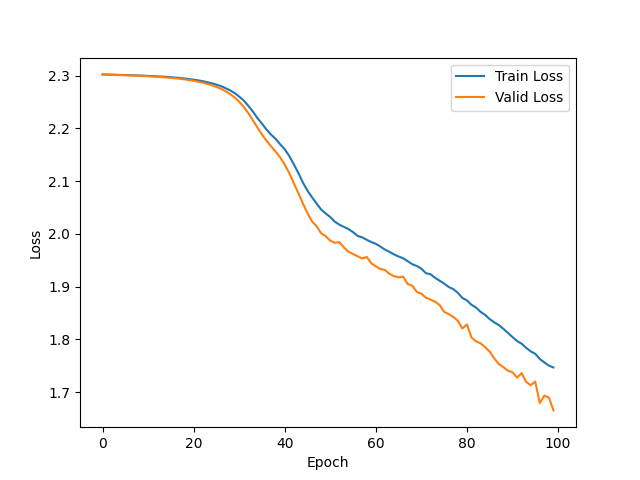
\includegraphics[width=1\linewidth]{Loss_1.5.png} &\vspace{5pt} 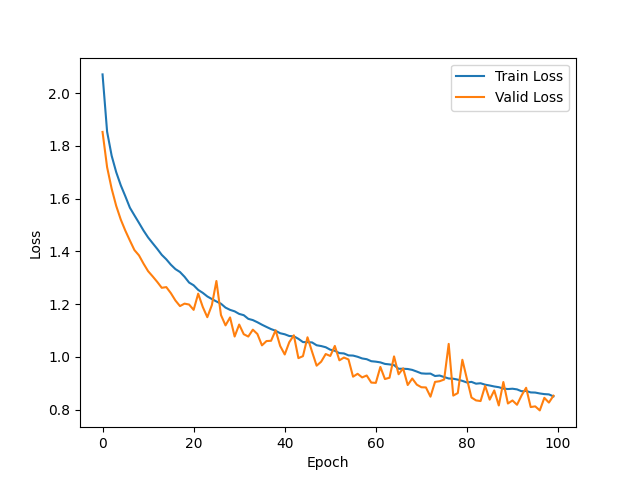
\includegraphics[width=1\linewidth]{Loss_2.png}  \\[0.6cm]
        \hline
        \begin{center} 2 \end{center}  &\vspace{5pt} 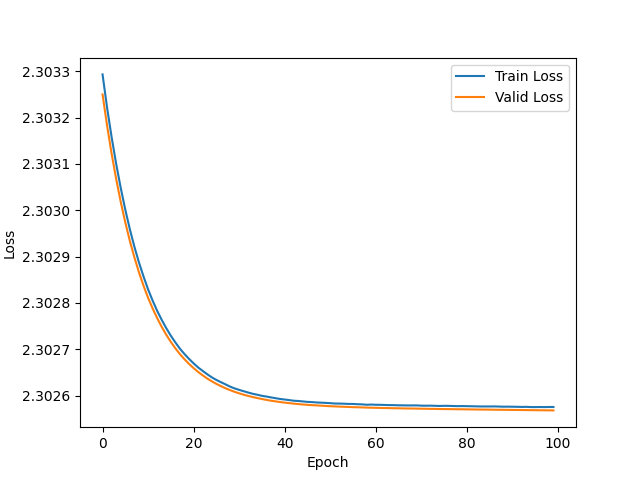
\includegraphics[width=1\linewidth]{Loss_4.5.png} &\vspace{5pt} 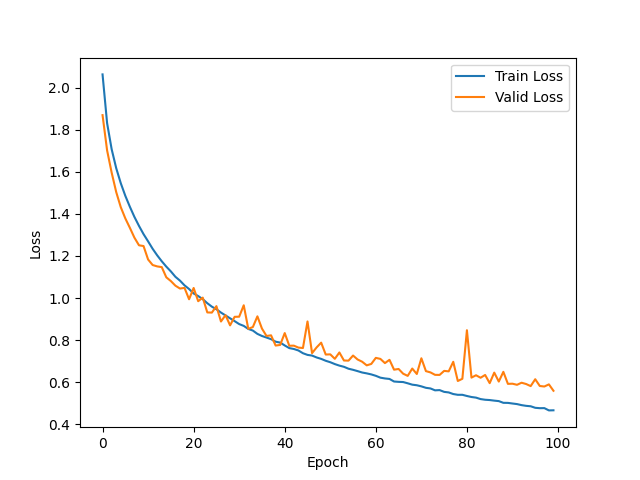
\includegraphics[width=1\linewidth]{Loss_5.png} \\[0.6cm]
        \hline
    \end{tabular}
    \caption{是否使用BatchNorm——Loss曲线}
\end{table}

\begin{table}[H]
    \centering
    \begin{tabular}{|m{1cm}|m{0.3\linewidth}|m{0.3\linewidth}|}
        \hline
        模型 &不使用BatchNorm函数 &使用BatchNorm函数\\[0.5cm]
        \hline
        \begin{center} 1 \end{center}  &\vspace{5pt} 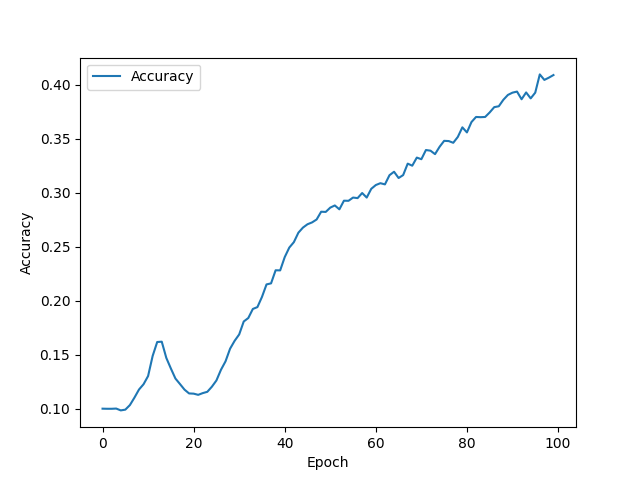
\includegraphics[width=1\linewidth]{Acc_1.5.png} &\vspace{5pt} 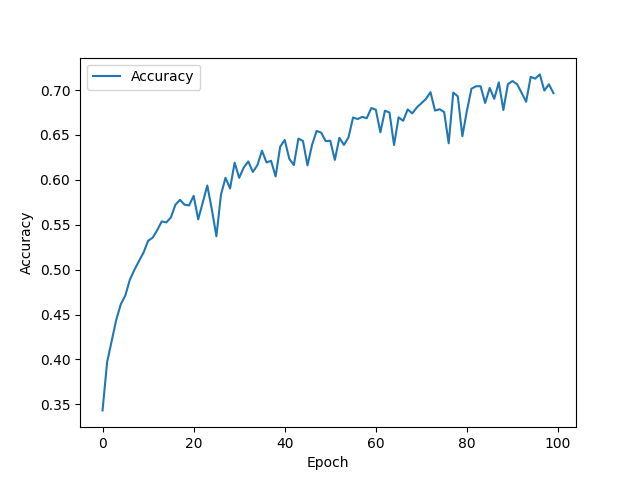
\includegraphics[width=1\linewidth]{Acc_2.png}  \\[0.6cm]
        \hline
        \begin{center} 2 \end{center}  &\vspace{5pt} 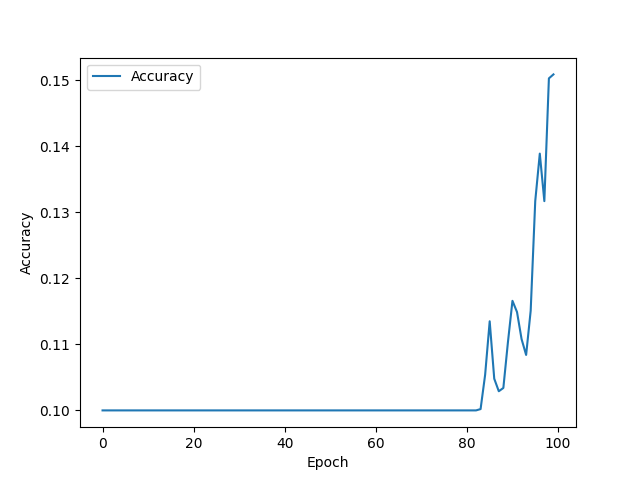
\includegraphics[width=1\linewidth]{Acc_4.5.png} &\vspace{5pt} 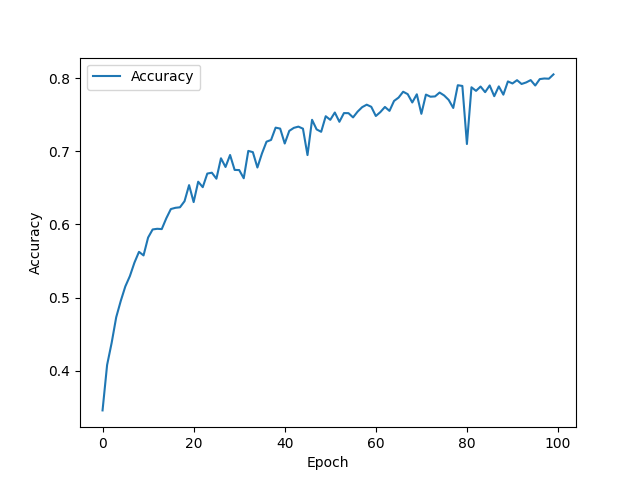
\includegraphics[width=1\linewidth]{Acc_5.png} \\[0.6cm]
        \hline
    \end{tabular}
    \caption{是否使用BatchNorm——Accuracy曲线}
\end{table}


对比使用 BatchNorm 和不使用 BatchNorm 的实验结果,可以看到在第 1 个较小的模型中,在使用
ReLU 函数的情况下,加入 BatchNorm 后,模型的准确率上升速度快速提升,且在训练集和测试集上的
表现差距变小。而在第 2 个较深的模型中,不使用 BatchNorm 时,模型在 100 个 epoch 内几乎没有学
习到任何东西,而使用 BatchNorm 后,模型在 100 个 epoch 内的准确率上升速度明显提升,训练效果
提升显著。这说明 BatchNorm 能够在较少的 epoch 内使模型趋向于收敛,且能够减小过拟合的风险。

同时根据激活函数的特点不同,对BatchNorm的依赖程度不同,可以知道BatchNorm可以将测试数据进行归一化
,从而起到加速训练、减小ReLU激活函数梯度消失问题、提高模型稳定性等作用。


\subsection{请根据结果分析更换优化器的效果}
使用不同优化器得到的训练结果如下:

\begin{table}[H]
    \centering
    \begin{tabular}{|m{1cm}|m{0.3\linewidth}|m{0.3\linewidth}|}
        \hline
        模型 &使用SGD优化器 &使用Adam优化器\\[0.5cm]
        \hline
        \begin{center} 1 \end{center}  &\vspace{5pt} 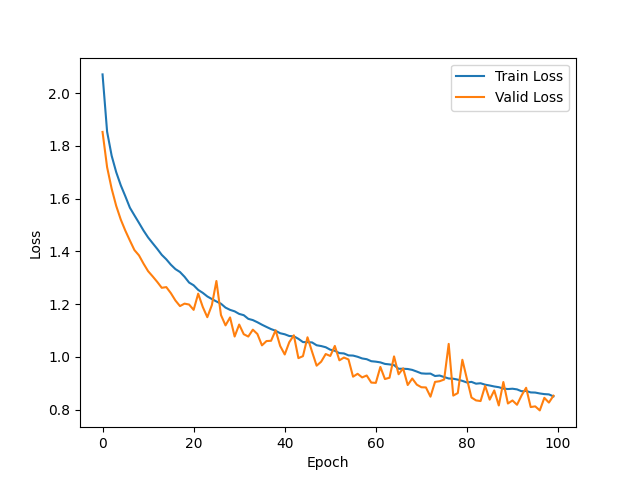
\includegraphics[width=1\linewidth]{Loss_2.png} &\vspace{5pt} 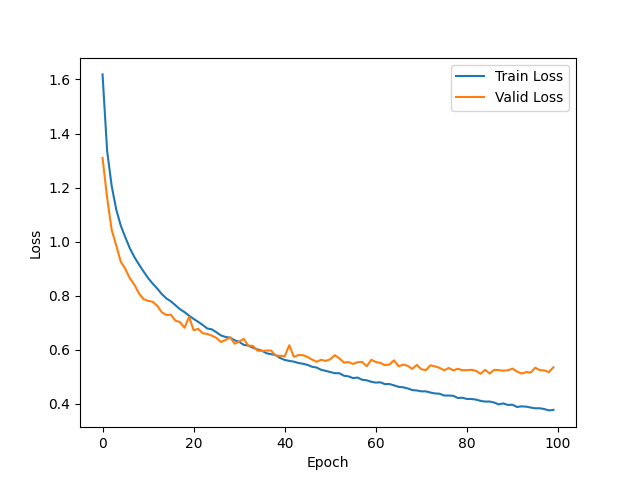
\includegraphics[width=1\linewidth]{Loss_3.png}  \\[0.6cm]
        \hline
        \begin{center} 2 \end{center}  &\vspace{5pt} 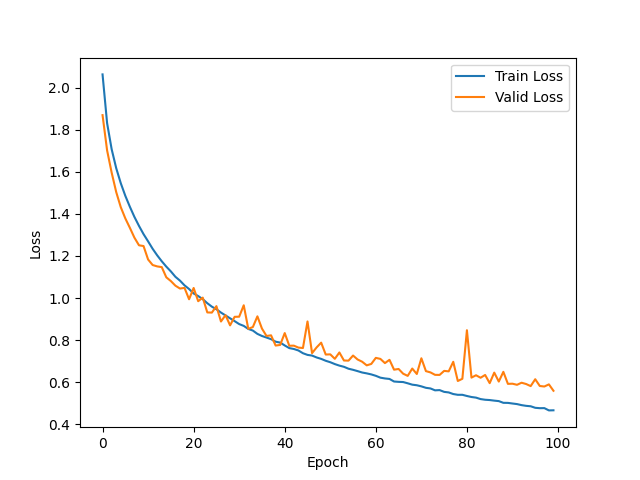
\includegraphics[width=1\linewidth]{Loss_5.png} &\vspace{5pt} 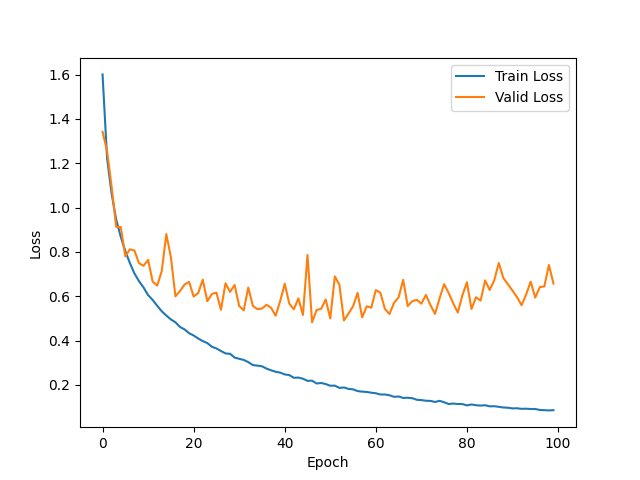
\includegraphics[width=1\linewidth]{Loss_6.png} \\[0.6cm]
        \hline
    \end{tabular}
    \caption{使用不同优化器——Loss曲线}
\end{table}

\begin{table}[H]
    \centering
    \begin{tabular}{|m{1cm}|m{0.3\linewidth}|m{0.3\linewidth}|}
        \hline
        模型 &使用SGD优化器 &使用Adam优化器\\[0.5cm]
        \hline
        \begin{center} 1 \end{center}  &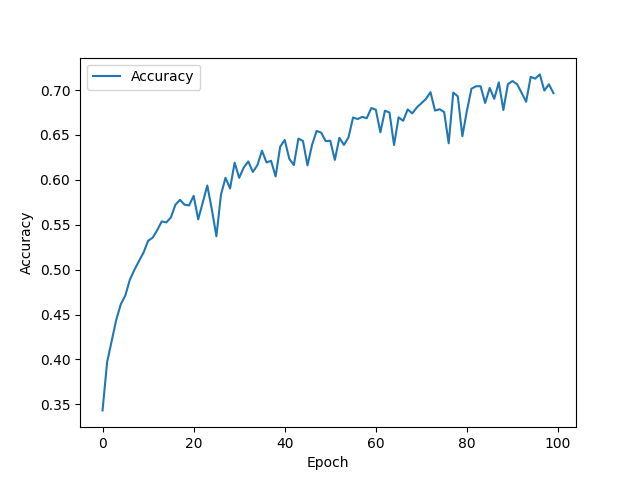
\includegraphics[width=1\linewidth]{Acc_2.png} &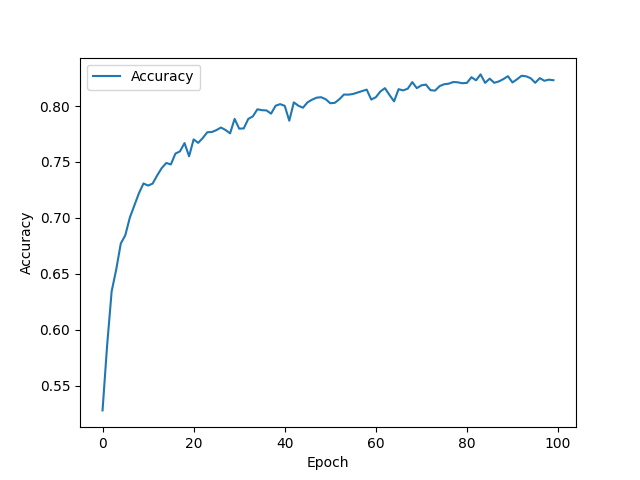
\includegraphics[width=1\linewidth]{Acc_3.png}  \\[0.6cm]
        \hline
        \begin{center} 2 \end{center}  &\vspace{5pt} 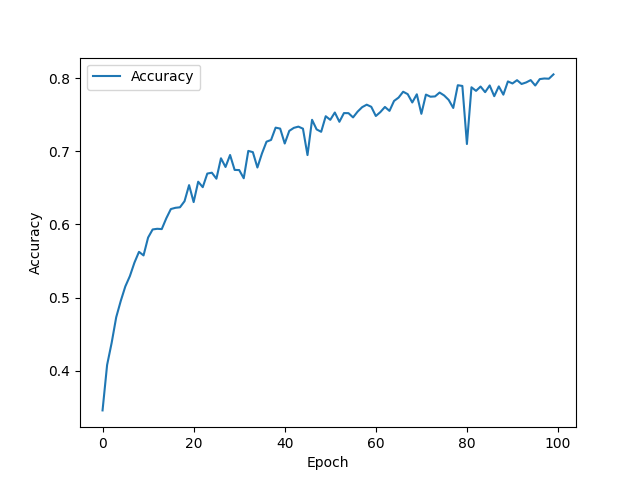
\includegraphics[width=1\linewidth]{Acc_5.png} &\vspace{5pt} 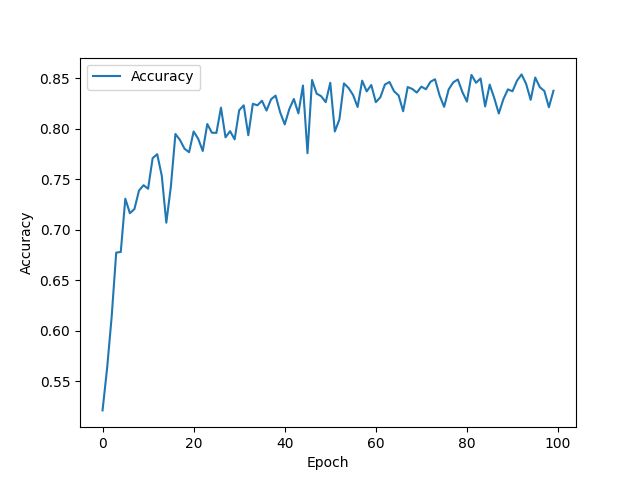
\includegraphics[width=1\linewidth]{Acc_6.png} \\[0.6cm]
        \hline
    \end{tabular}
    \caption{使用不同优化器——Accuracy曲线}
\end{table}

对比使用 SGD 和使用 Adam 的实验结果,可以看到将优化器从 SGD 更换为 Adam 后,模型的准确率能
够在较少的 epoch 内达到较高的水平,曲线也更加平滑。在 100 个 epoch 内,Adam 优化器的模型准
确率明显高于 SGD 优化器的模型准确率。但是可以发现,到后期 Adam 的验证集 Loss 曲线显著高于训
练集 Loss 曲线,难以下降,这可能是由于过拟合导致的。

这是因为 Adam 的自适应性学习率能够使模型在训练过程中更快地收敛,且能够避免 SGD 的学习率过
大导致的梯度震荡现象。Adam 倾向于更快地收敛,但也可能更容易陷入过拟合。在训练后期,它可能
会过快地找到局部最优解,导致模型的泛化能力下降。

\subsection{请根据你的结果分析模型是否出现了过拟合,如有,请在图像中指出在哪里出现了
过拟合。如无,请给出你判断的原因}
实验4过程中确实出现了过拟合,如下图
\begin{figure}[H]
    \centering
    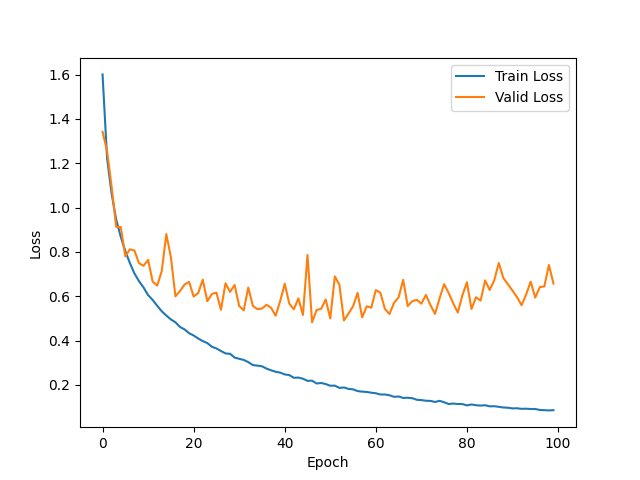
\includegraphics[width=0.6\linewidth]{Loss_6.png}
    \caption{实验4更换为Adam优化器后Loss曲线}
\end{figure}

实验1到3几乎都没有出现过拟合的情况。实验4中使用SGD优化时过拟合现象也不明显。但是
在实验 4 将优化器切换为 Adam 优化器后,模型出现了明显的过拟合。验证集的 Loss 几乎保持不变, 
而训练集的 Loss 在后期持续下降,这说明模型在训练集上表现良好,但在验证集上表现较差,即模型出 
现了过拟合。

\newpage
\begin{appendices}
\section*{附录}
\section{代码填空}
\subsection*{DeepNet}
\begin{lstlisting}
class DeepNet(nn.Module):
    def __init__(self, act):
        super(DeepNet, self).__init__()
        ################### 代码填空:请在此填补模型定义代码 ###################
        self.conv1 = nn.Conv2d(3, 16, 3, padding=1)
        self.conv2 = nn.Conv2d(16, 32, 3, padding=1)
        self.pool1 = nn.MaxPool2d(2, 2)
        self.conv3 = nn.Conv2d(32, 64, 3, padding=1)
        self.conv4 = nn.Conv2d(64, 128, 3, padding=1)
        self.pool2 = nn.MaxPool2d(2, 2)
        self.conv5 = nn.Conv2d(128, 256, 3, padding=1)
        self.conv6 = nn.Conv2d(256, 512, 1, padding=0)
        self.pool3 = nn.AdaptiveAvgPool2d((1, 1))
        self.fc1 = nn.Linear(512, 256)
        self.fc2 = nn.Linear(256, 128)
        self.fc3 = nn.Linear(128, 10)
        if act == 'relu':
            self.act = F.relu
        elif act == 'tanh':
            self.act = F.tanh
        elif act == 'sigmoid':
            self.act = F.sigmoid
        ##################################################################

    def forward(self, x):
        # convolutional layers
        ################### 代码填空:请在此填补前向计算代码 ###################
        x = self.pool1(self.act(self.conv2(self.act(self.conv1(x)))))
        x = self.pool2(self.act(self.conv4(self.act(self.conv3(x)))))
        x = self.pool3(self.act(self.conv6(self.act(self.conv5(x)))))
        x = x.view(-1, 512)
        x = self.act(self.fc1(x))
        x = self.act(self.fc2(x))
        x = self.fc3(x)
        return x
        ##################################################################
        pass
\end{lstlisting}
\subsection*{BnDeepNet}
\begin{lstlisting}
class BnDeepNet(nn.Module):
    def __init__(self,act):
        super(BnDeepNet, self).__init__()
        ################### 代码填空:请在此填补模型定义代码 ###################
        self.conv1 = nn.Conv2d(3, 16, 3, padding=1)
        self.bn1 = nn.BatchNorm2d(16)
        self.conv2 = nn.Conv2d(16, 32, 3, padding=1)
        self.bn2 = nn.BatchNorm2d(32)
        self.pool1 = nn.MaxPool2d(2, 2)
        self.conv3 = nn.Conv2d(32, 64, 3, padding=1)
        self.bn3 = nn.BatchNorm2d(64)
        self.conv4 = nn.Conv2d(64, 128, 3, padding=1)
        self.bn4 = nn.BatchNorm2d(128)
        self.pool2 = nn.MaxPool2d(2, 2)
        self.conv5 = nn.Conv2d(128, 256, 3, padding=1)
        self.bn5 = nn.BatchNorm2d(256)
        self.conv6 = nn.Conv2d(256, 512, 1, padding=0)
        self.bn6 = nn.BatchNorm2d(512)
        self.pool3 = nn.AdaptiveAvgPool2d((1, 1))
        self.fc1 = nn.Linear(512, 256)
        self.bn7 = nn.BatchNorm1d(256)
        self.fc2 = nn.Linear(256, 128)
        self.bn8 = nn.BatchNorm1d(128)
        self.fc3 = nn.Linear(128, 10)
        if act == 'relu':
            self.act = F.relu
        elif act == 'tanh':
            self.act = F.tanh
        elif act == 'sigmoid':
            self.act = F.sigmoid
        ###################################################################

    def forward(self, x):
        # convolutional layers
        ################### 代码填空:请在此填补前向计算代码 ###################
        x = self.pool1(self.act(self.bn2(self.conv2(self.act(self.bn1(self.conv1(x)))))))
        x = self.pool2(self.act(self.bn4(self.conv4(self.act(self.bn3(self.conv3(x)))))))
        x = self.pool3(self.act(self.bn6(self.conv6(self.act(self.bn5(self.conv5(x)))))))
        x = x.view(-1, 512)
        x = self.act(self.bn7(self.fc1(x)))
        x = self.act(self.bn8(self.fc2(x)))
        x = self.fc3(x)
        return x
        ##################################################################
        pass
\end{lstlisting}

\subsection*{Optimizer}
\begin{lstlisting}
optimizer_type = "SGD" #或者换成AdamW
    if optimizer_type == "SGD":
    optimizer = optim.SGD(model.parameters(), lr=0.001)
elif optimizer_type == "Adam":
    ########## 代码填空:请在此填补Adam优化器计算代码, lr=0.0001 ###########
    optimizer = optim.Adam(model.parameters(), lr=0.0001)
    ##################################################################
    pass
\end{lstlisting}
\end{appendices}
\end{document}
